\section{System Design}

This chapter presents a detailed account of the design of the GenAI Advisor system, designed to deliver explainable, user-friendly financial insights for retail investors with an interest in Generative AI equities.

\subsection{System Overview \& Design Rationale}

The architecture of the GenAI Advisor system is composed of five distinct yet interdependent layers:

\begin{enumerate}
    \item \textbf{Data Pipeline}, responsible for sourcing, cleaning, and transforming financial data into formats suitable for analysis.
    \item \textbf{Strategy Engine}, the analytical core that integrates retrieved knowledge to generate structured investment insights.
    \item \textbf{Explanation Generator}, producing justifications and rationales for each recommendation.
    \item \textbf{User Interface}, delivers an intuitive interaction point for retail users, visualising results in a digestible and accessible format.
    \item \textbf{Backtesting \& Evaluation}, supports validation of generated recommendations through historical simulations, user feedback loops and performance scoring.
\end{enumerate}

Each layer encapsulates a single responsibility while remaining interoperable with adjacent layers, reflecting a separation-of-concerns design philosophy. This modular approach enables independent development and testing of each component, reducing coupling and simplifying future iterations or extensions.

\begin{figure}[ht]
    \centering
    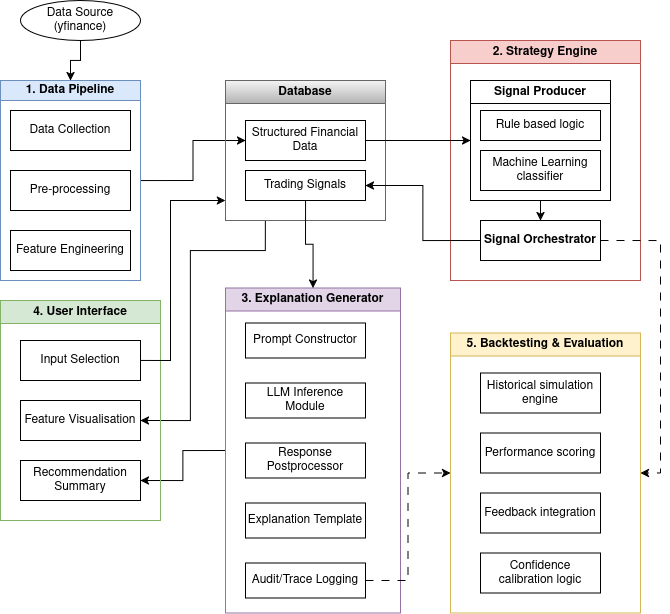
\includegraphics[width=0.5\textwidth]{assets/systemDesign.png}
    \caption{Five-layer Architecture of GenAI Advisor}
    \label{fig:systemDesign}
\end{figure}

The design rationale also reflects broader system requirements, particularly the need for explainability, adaptability, and integration with real-time financial data streams. Embedding traceability into the architecture ensures that every recommendation is grounded in verifiable data sources, supporting responsible AI usage. Furthermore, by situating the explanation generator as a distinct layer, the architecture highlights the importance of user trust and transparency as core design principles.

Scalability is not a goal of the current system, and no scaling mechanisms will be implemented in either the prototype or the final version. However, scalability remains an important consideration in the broader context of deploying AI systems in production environments. Should the system be developed further, future work could explore stateless service design, containerised deployment, and asynchronous processing to support larger data volumes and concurrent users. Flexibility across infrastructure backends and compatibility with different classes of language models could also be considered to enable wider applicability.

\subsection{Data Pipeline}

This foundational layer is responsible for acquiring, preparing, and transforming financial data into structured formats that support both retrieval and modelling. It ensures that the inputs to the system are consistent and semantically rich.

\textbf{Data Sources:} Financial data is sourced via the \texttt{yfinance} Python library, which extracts structured data from Yahoo Finance. This includes:
\begin{itemize}
    \item Daily price data
    \item Adjusted close prices accounting for dividends and splits
    \item Market fundamentals including P/E ratio, EPS, market capitalisation, and beta
    \item Dividend history, earnings results, and analyst forecasts
    \item Corporate actions such as stock splits and ex-dividend dates
\end{itemize}

\textbf{Pre-processing:} All raw data is immediately pre-processed in memory using \texttt{pandas} and associated libraries before being persisted. This includes:
\begin{itemize}
    \item Handling of missing values and filtering of anomalous entries
    \item Normalisation and transformation of numerical columns
    \item Resampling and forward-filling to align time indices across features
    \item Annotating rows with relevant metadata
\end{itemize}
This pre-processing ensures consistency across all instruments and time periods and reduces computational load in downstream stages.

\textbf{Data Storage:} Once cleaned and transformed, the processed dataset is stored in a relational MariaDB database. This allows for fast, structured access by subsequent system components and avoids repeated API calls to Yahoo Finance. Tables are designed to support efficient filtering by date, ticker, and feature type. Indexes are maintained on primary keys and time columns to optimise query latency.

\textbf{Feature Engineering:} This stage derives higher-order signals and representations from the cleaned data:
\begin{itemize}
    \item \textbf{Technical indicators:} including moving averages, MACD, RSI, and volatility bands
    \item \textbf{Fundamental deltas:} e.g. growth rates in earnings, changes in valuation multiples
    \item \textbf{Risk signals:} calculated from rolling variance, beta, and return dispersion
    \item \textbf{Embeddings:} tabular records are converted into dense vector representations using Sentence-BERT for semantic similarity and retrieval
\end{itemize}

\textbf{Design Justification:} The choice of MariaDB for structured data storage reflects a balance between transparency, performance, and system complexity. Relational databases offer well-defined schema enforcement, support for indexed queries, and seamless integration with Python data analysis libraries. This aligns with the project's emphasis on explainability, traceability, and reproducibility. Alternative solutions were considered, including DuckDB for embedded analytics or Parquet-backed storage for columnar efficiency. However, these options introduce either added complexity or are optimised for larger-scale, concurrent systems. For the scope of this project, focusing on iterative prototyping, backtesting, and clarity, MariaDB provides a robust and pedagogically sound foundation.

\subsection{Strategy Engine}

The strategy engine forms the analytical core of the GenAI Advisor system, responsible for evaluating investment opportunities using structured signals and domain-specific rules. It interprets features derived from historical data and generates intermediate outputs such as buy/sell/hold flags, risk scores, and confidence levels. This layer operates independently of any generative model.

\textbf{Signal Retrieval:} At runtime, the strategy engine queries the MariaDB backend for time-aligned features such as technical indicators, valuation metrics, volatility profiles, and momentum scores. Data is filtered by ticker, date, and sector using predefined criteria. Missing values are handled via forward-filling or exclusion depending on the indicator’s sensitivity.

\textbf{Rule-based Scoring:} Initial decision logic is implemented using deterministic rules. For example:
\begin{itemize}
    \item \emph{Momentum signal:} Generate a buy signal if the closing price exceeds the 50-day simple moving average and RSI is in the range 50–70.
    \item \emph{Valuation screen:} Flag as overvalued if the P/E ratio is greater than the sector median by more than one standard deviation.
    \item \emph{Risk classification:} Assign a “high risk” label if beta exceeds 1.5 or if recent earnings variance is above a defined threshold.
\end{itemize}
These rule sets are configurable and grounded in established financial heuristics.

\textbf{Machine Learning Models:} Where applicable, supervised models such as logistic regression or gradient-boosted decision trees may be used to estimate directional signals. Input features include moving averages, volatility, return profiles, and sector-adjusted valuation ratios. Outputs are binary or probabilistic classifications of investment suitability.

\textbf{Strategy Output:} The final output is a structured intermediate recommendation, for example:
\begin{itemize}
    \item \emph{Ticker:} MSFT
    \item \emph{Action:} HOLD
    \item \emph{Confidence:} 72\%
    \item \emph{Tags:} “Moderate Risk”, “Overvalued”
\end{itemize}
This output is passed to the explanation layer, where it is contextualised and communicated to the end-user through a natural language interface.

The strict separation of decision logic from explanation ensures that recommendations are reproducible and auditable across time.

\subsection{Explanation Generator}

The explanation generator is responsible for converting structured strategy outputs into human-readable narratives. This layer interfaces with a large language model (LLM) to articulate the rationale behind each recommendation, ensuring the system remains explainable, and transparent.

\textbf{Prompt Construction:} Each recommendation generated by the strategy engine is converted into a structured prompt. This prompt contains:
\begin{itemize}
    \item The recommended action (e.g. BUY, HOLD, SELL)
    \item Associated features (e.g. P/E ratio, RSI, volatility)
    \item Descriptive tags (e.g. “Overvalued”, “Moderate Risk”)
    \item Ticker metadata (e.g. sector, market cap, recent price movement)
\end{itemize}
The prompt template enforces a consistent narrative structure and ensures that only relevant, pre-computed data is surfaced to the LLM. No raw retrieval or document inference is performed at this stage.

\textbf{LLM Invocation:} The prompt is submitted to a locally hosted language model, with inference restricted to models that can be executed on a GPU with 8GB of VRAM. This design constraint promotes offline operability.

\textbf{Post-processing and Attribution:} The LLM output is parsed and linked to its underlying features. Numerical drivers are tagged and cross-referenced with the original strategy inputs to enable traceability. Where applicable, confidence indicators and relevant feature values are surfaced alongside the textual response.

\textbf{Model Selection Rationale:} For the purpose of this project, fine-tuning large language models is deliberately excluded due to its high resource demands and limited added value in the context of structured explanation generation. Instead, the system leverages pre-trained models served locally via the Ollama framework, which supports quantised variants of open-source architectures such as Mistral, Phi-2, and LLaMA2. These models strike a practical balance between performance and hardware feasibility, running comfortably on an 8GB VRAM GPU. The focus is placed on prompt design and response evaluation rather than model adaptation. This strategy aligns with the project’s emphasis on transparency and reproducibility, while avoiding the complexity and risks associated with custom model training.

By isolating the explanation function from decision-making logic and constraining it to local, auditable models, this design ensures the advisory system remains intelligible, trustworthy, and compliant with practical deployment constraints.

\subsection{User Interface}

The user interface (UI) serves as the primary point of interaction between the end-user and the advisory system. It is designed to surface system outputs in a clear and context-aware format while abstracting away the technical complexity of the underlying architecture.

\textbf{Interface Design Principles:} The UI is guided by the principles of usability, transparency, and minimalism. It aims to provide information density without cognitive overload, and supports both exploratory queries and structured evaluations.

\textbf{Interaction Model:} The primary mode of interaction is a ticker selector and a time window. Queries are routed through the backend pipeline and responses are returned in astructured, explanation-rich format.

\textbf{Presentation Layer:} Output is displayed in modular response cards, with each card corresponding to a company. Each card includes:
\begin{itemize}
    \item The recommended action (BUY, HOLD, SELL)
    \item A summarised rationale generated by the explanation layer
    \item Key features (e.g. P/E ratio, RSI, beta) highlighted inline
    \item Option to expand for full explanation and numerical context
\end{itemize}
Cards are sorted based on confidence or relevance, and users can collapse or pin cards for comparison.

\textbf{Technical Implementation:} The frontend is built using a lightweight web framework such as Streamlit. This ensures rapid prototyping, cross-platform compatibility, and support for secure API calls to backend services. The UI is deployed as a local web application accessible via browser.

\textbf{Responsiveness and Accessibility:} The interface is optimised for both desktop and mobile devices. Layouts use responsive containers and typography is chosen for readability. Accessibility guidelines such as contrast ratios and semantic labelling are followed to ensure inclusivity.

This interface completes the user-facing layer of the system, enabling seamless communication of insights derived from structured analysis and local language model generation.

\subsection{Backtesting \& Evaluation}

This layer is responsible for assessing the performance, consistency, and interpretability of the GenAI Advisor system. Evaluation is conducted along two axes: (i) financial effectiveness of the recommendations and (ii) fidelity and stability of the generated explanations.

\textbf{Backtesting of Strategy Output:} The system supports retrospective evaluation of strategy outputs using historical financial data stored in MariaDB. Given a time window and a set of tickers, the engine replays strategy decisions based on data available at the time. The simulated trades are benchmarked using standard performance metrics such as:
\begin{itemize}
    \item Cumulative return
    \item Sharpe ratio
    \item Maximum drawdown
    \item Hit rate (proportion of correct directional calls)
\end{itemize}
These simulations validate whether the rule-based and ML-driven components produce economically viable signals under realistic conditions.

\textbf{Evaluation of Explanation Consistency:} Because the system includes a generative component, it is essential to assess the consistency and fidelity of explanations. For a given strategy output, repeated LLM invocations are evaluated for semantic agreement and factual stability. Techniques include:
\begin{itemize}
    \item \emph{Stability under identical prompts:} The same input is submitted multiple times to check for drift.
    \item \emph{Paraphrase testing:} Slightly altered prompts are compared for explanation robustness.
    \item \emph{Key fact alignment:} Extracted metrics in the explanation are compared against known strategy outputs.
\end{itemize}
These tests ensure that the narrative remains faithful to the underlying numerical reasoning.

\textbf{User Feedback Loop:} The UI logs user reactions to recommendations through binary feedback (e.g. thumbs up/down). Feedback is stored with associated prompt and strategy metadata, enabling post-hoc review and potential retraining of classification thresholds or strategy weights.

\textbf{Qualitative Auditing:} In addition to automated tests, a sample of responses is manually audited to assess:
\begin{itemize}
    \item Clarity of the natural language explanation
    \item Justification coverage (i.e., do the reasons align with the action?)
    \item Absence of hallucinated content or misleading terminology
\end{itemize}
This step supports ethical AI principles by ensuring outputs remain comprehensible and appropriate for retail consumption.

This evaluation layer closes the loop between system logic, narrative explanation, and end-user experience. It provides the foundations for continuous improvement while maintaining interpretability and trust.
